\section{Практична частина}
\setlength{\parindent}{4em}
\begin{center}
  {\textbf{\emph{Схема 1}}}
\end{center}
\begin{figure}[ht]

\centering

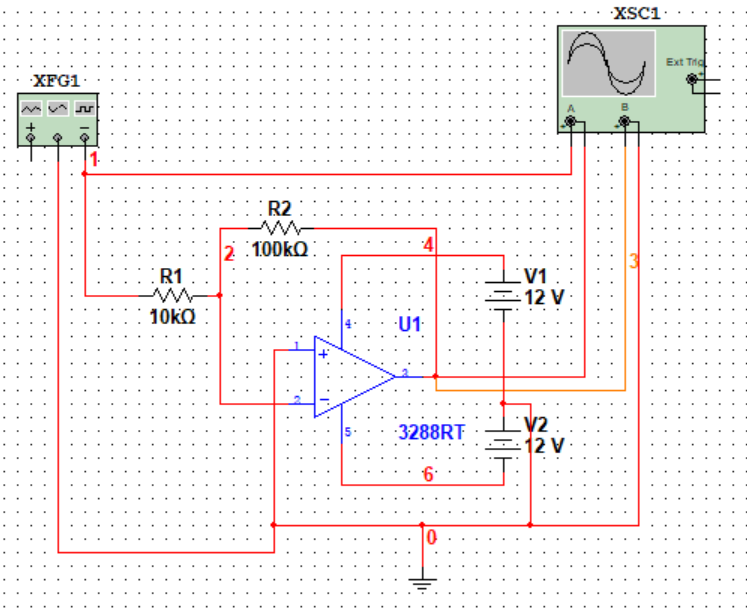
\includegraphics[width=0.7\linewidth]{Pic/circuit_1_screen.png}

\caption{Перша схема з використанням підсилювача}

\label{Prac1}

\end{figure}
\begin{figure}[ht]

\centering

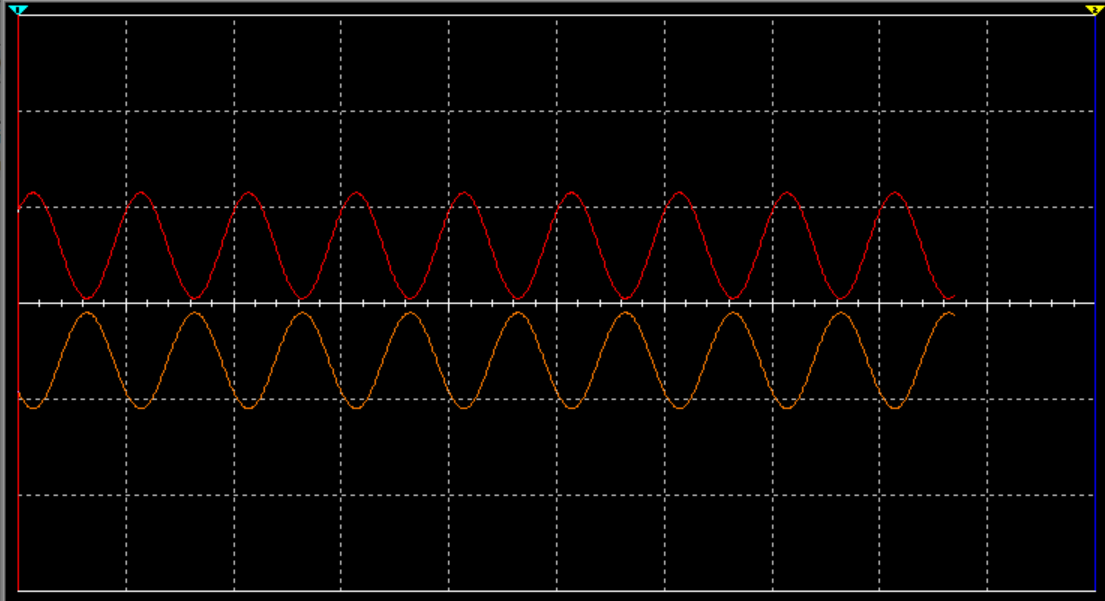
\includegraphics[width=0.7\linewidth]{Pic/circuit_1_plot.png}

\caption{Отримана напруга на вході та на виході}

\label{Prac2}

\end{figure}
\newpage
\begin{center}
  {\textbf{\emph{Схема 2}}}
\end{center}
\begin{figure}[ht]

\centering

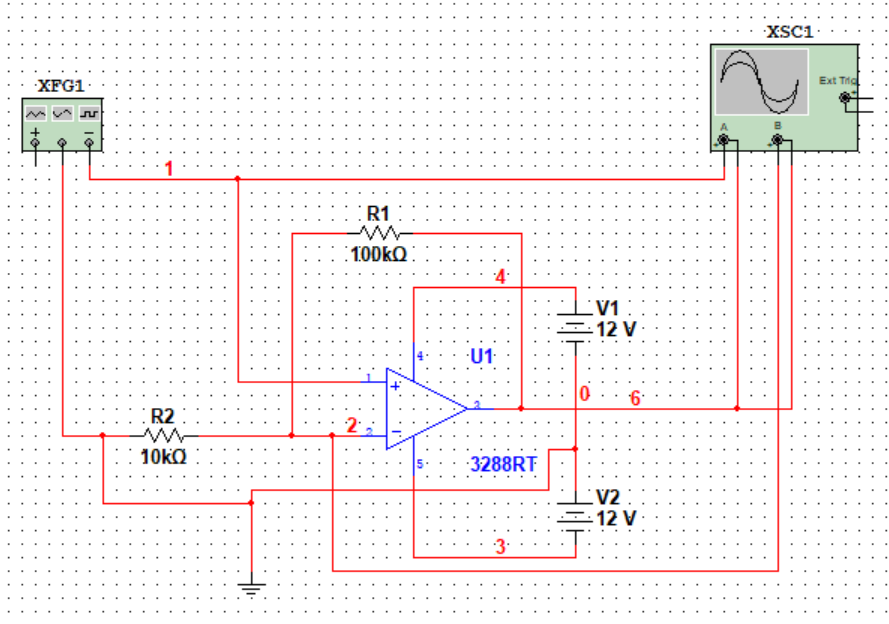
\includegraphics[width=0.7\linewidth]{Pic/circuit_2_screen.png}

\caption{Друга схема з використанням підсилювача}

\label{Prac3}

\end{figure}
\begin{figure}[ht]

\centering

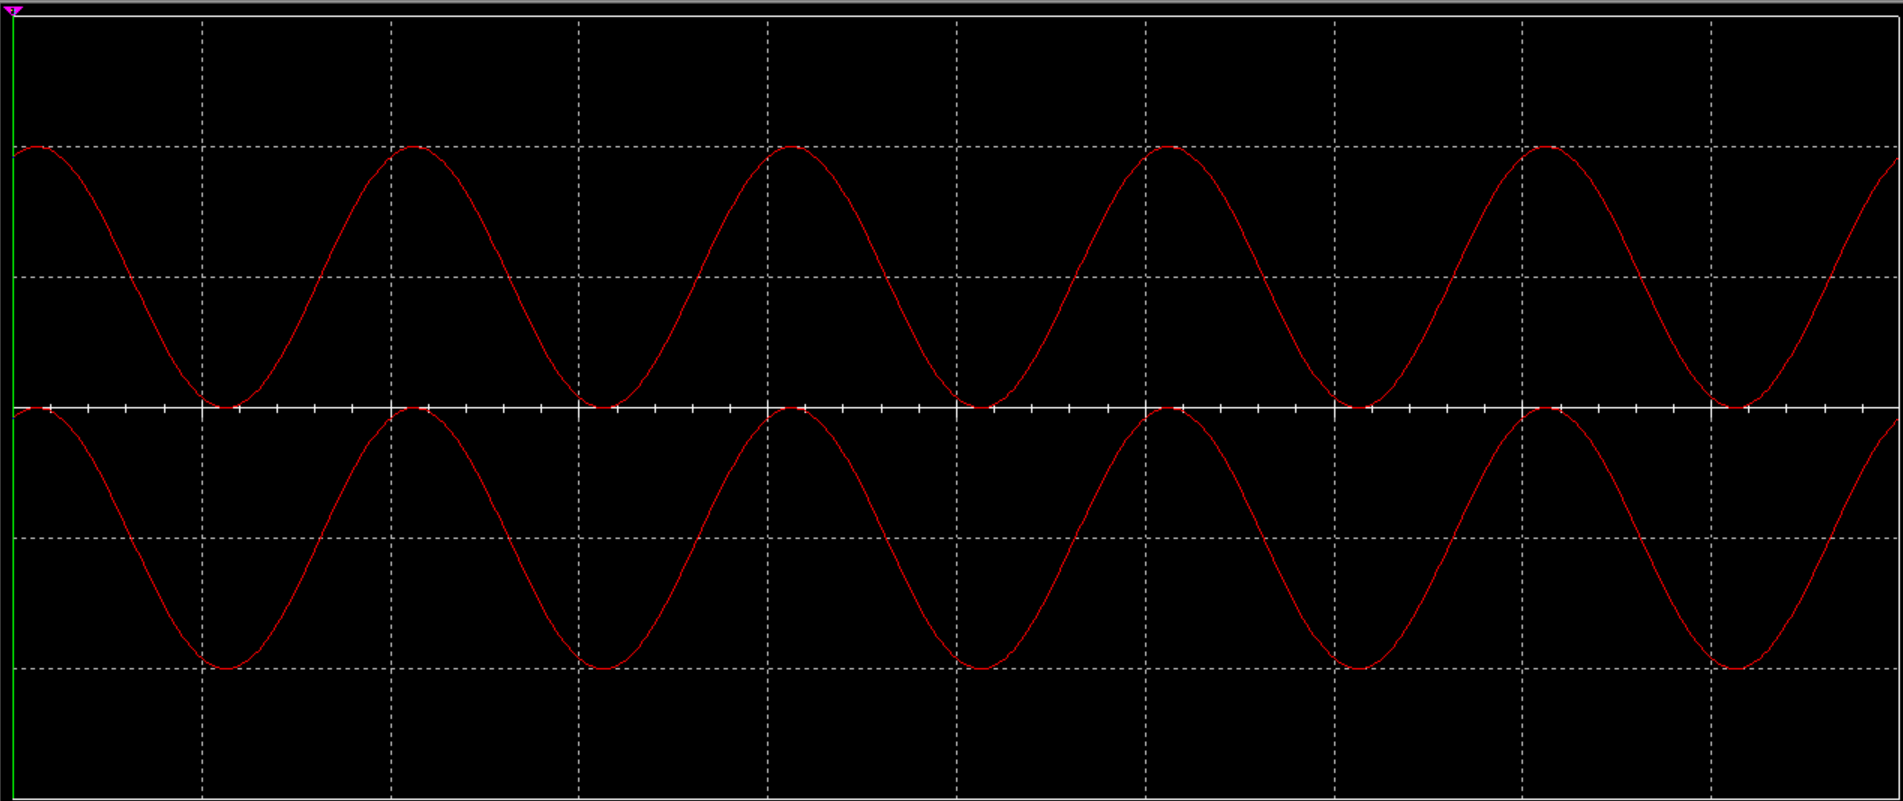
\includegraphics[width=0.7\linewidth]{Pic/circuit_2_plot.png}

\caption{Отримана напруга на вході та на виході}

\label{Prac4}

\end{figure}
\newpage
\begin{center}
  {\textbf{\emph{Схема 3}}}
\end{center}
\begin{figure}[ht]

\centering

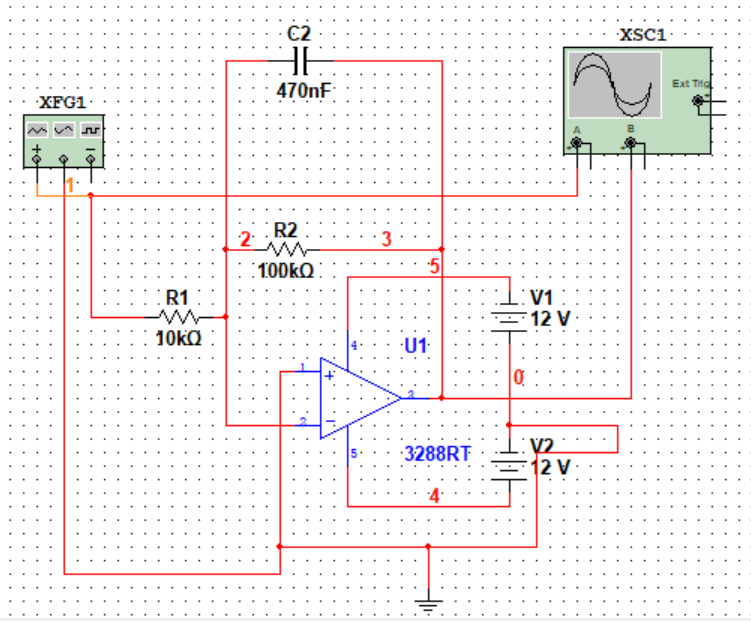
\includegraphics[width=0.7\linewidth]{Pic/circuit_3_screen.png}

\caption{Третя схема з використанням підсилювача}

\label{Prac1}


\end{figure}
\begin{figure}[ht]

\centering

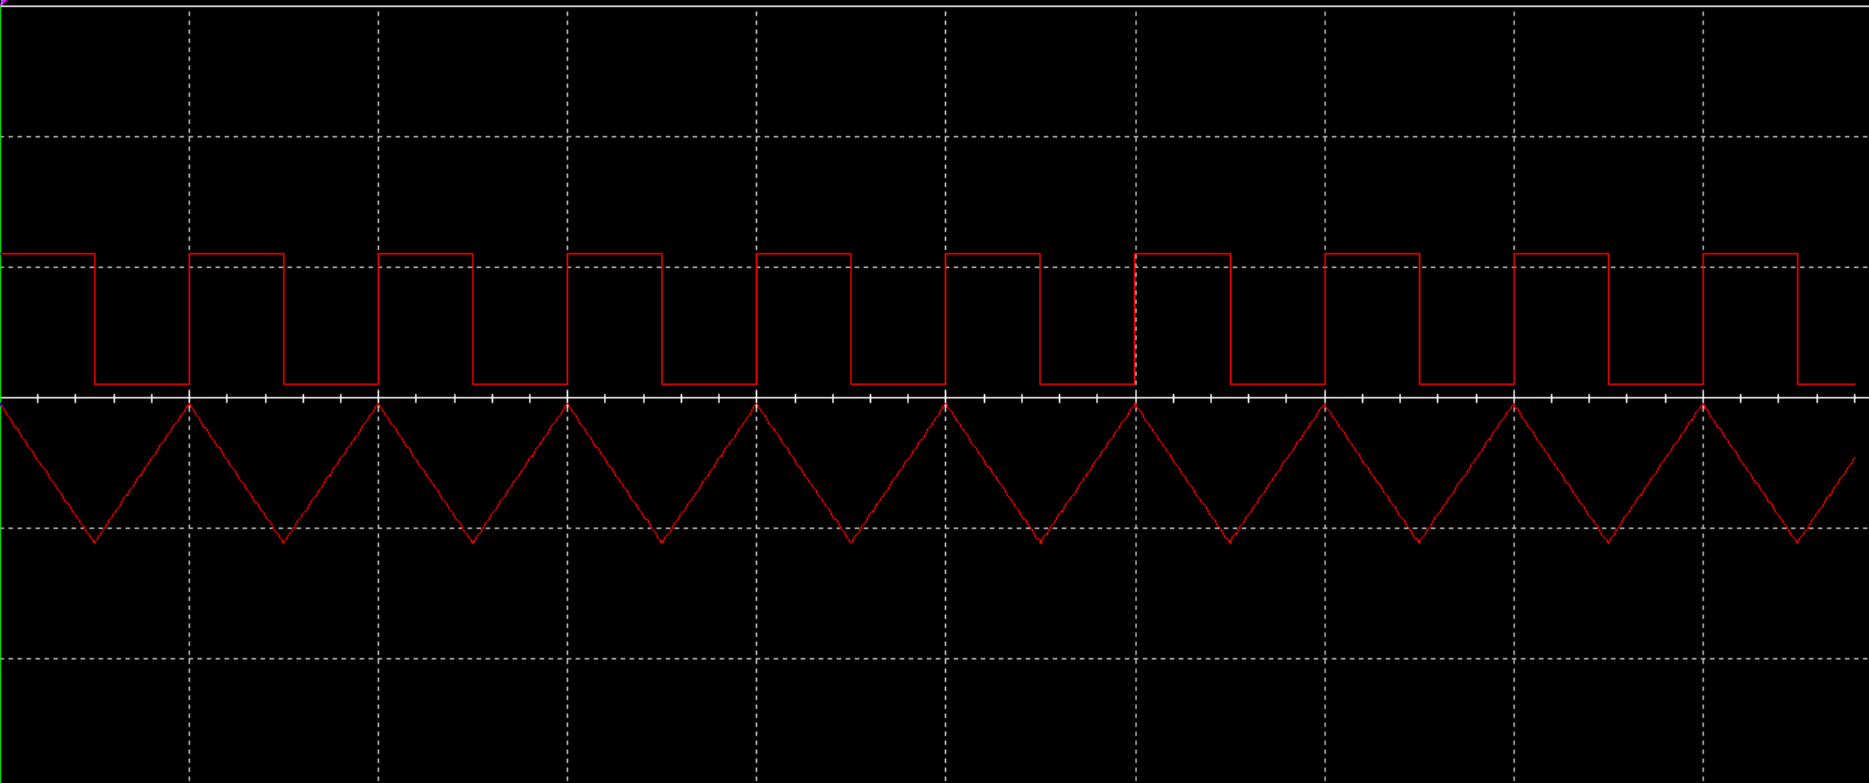
\includegraphics[width=0.7\linewidth]{Pic/circuit_3_plot.png}

\caption{Отримана напруга на вході та на виході}

\label{Prac1}

\end{figure}

\newpage
